\section{Results}
\label{sec:results}
\David{The text in this section feels like you are trying to find content by adding methods and discussion.  Don't give in to that temptation.  Result sections are short and should be mostly figures and tables.  I added some ideas of what else to discuss below.}

\David{I feel your results should start with what is obvious to you: IT WORKS. It converges.  You get a result. The result can predict behavior with an accuracy of XYZ.  It took x long to get this result.  If you used different seeds, you always get the same answer (because linear fitting).  Don't forget that you are doing this for the first time and it is important to note that it works.  People will ask themselves how well it works and how they can use it.  Do you need to tune stuff?  Do you need to carefully select parameters or initial guesses?}

\David{Similar, you can discuss the same properties for the other models and identification processes.  My guess would be that for some of the nonlinear methods your result depend on the initial guess and might vary.}

\David{Can you quantify the level of `non-linearity' of your robot?  This would be very valuable for a reader who wants to understand if this nonlinear approach is even necessary.  Can you discuss which of the other methods are linear/ nonlinear.}

\David{While all your results are presented in tables and figures, you should summarize and quantify the main results.  e.g.:  Your approach has an RSME of XYZ.  Your approach outperforms the best nonlinear model by XYZ\%.  it outperforms the best linear model by XYZ\%. It took XYZ seconds to find a solution.  etc.}

%% FIGURE: Koopman simulation plot
\begin{figure}
    \centering
    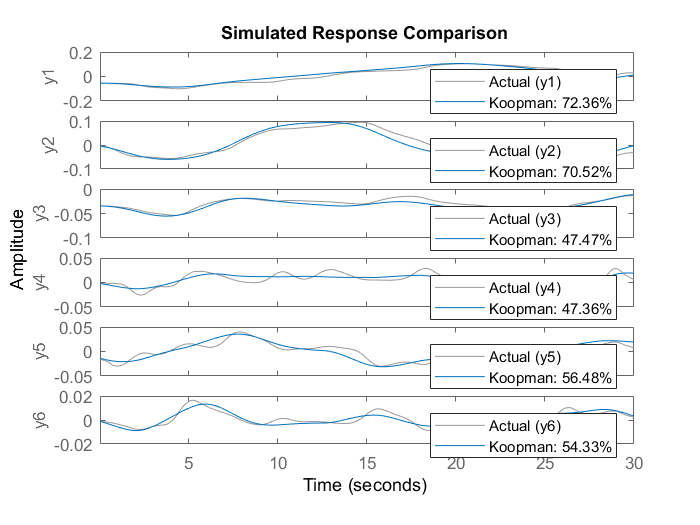
\includegraphics[width=\linewidth]{figures/koopPlot_ph1.png}
    \caption{PLACEHOLDER: Simulation of model generated by Koopman system identification technique verses real system.
    Simulation of the model generated by the Koopman sysid method (blue) superimposed with the measured behavior of the system (grey) over a 30 second time window given the same initial condition and control inputs. The NRMSE for each state is shown in the boxes on the right. \Ram{Please label the y-axis in each plot appropriately. It maybe worth comparing at least one other prediction generated from another sys id technique. Please color everything the same way, consistently (e.g. blue is Koopman, purple is n.n., etc.). Given space restrictions we may want to show another prediction as well. I'd remove the NRMSE from the plot. }}
    \label{fig:koopmanSim}
\end{figure}


%% Performance was evaluated by comparing simulations to real measurements
A state space model was generated from the technique described in section \ref{sec:theory} using a monomial basis of maximum degree $w=3$.
We evaluated its accuracy by comparing model simulations to validation data (Fig. \ref{fig:koopmanSim}).
Goodness of fit for the trajectory of a state $y$ was calculated using the normalized root-mean-square error (NRMSE)
%% Normalized Root Mean-Square Error
\aln{
    \text{NRMSE} &= \frac{\text{RMSE}}{y_\text{max} - y_\text{min}} \\
    \text{RMSE} &= \sqrt{ \frac{\sum_{k=1}^{N_\text{total}} \left( y_k - \hat{y}_k \right)^2}{N_\text{total}} }
    % 1 - \frac{ \| y - \hat{y}  \| }{ \| y - \text{mean}(y) \| }
}
where $\hat{y}$ is the simulated value of the state, $N_\text{total}$ is the total number of points, and $y_{\text{min/max}}$ are the measured maximum/minimum values of the state observed over all trials.
% A NRMSE of $1$ denotes a perfect fit, while a value less than or equal to $0$ implies that the model output is no better than a straight line at fitting the validation data.

%% For comparison, other sysid methods were also used on the same set of data
The performance of our model was benchmarked against several other models that were generated using the Matlab System Identification Toolbox and Neural Network Toolbox \cite{MATLAB:2017}.
\David{I know this information is in the table, but i would also specify in the text.  ALSO: I would strongly suggest to make this part of methods.  Add a  subsection D ``Model comparison'' and describe these other models there.}
These models were trained on the same data set as the Koopman model, 
Then, the models were simulated under the same inputs as those from the validation trials described in section \ref{sec:experiment}.
\David{Condense: ``All models were trained and evaluated on the same training and evalution data.''} \David{also: move to methods.}
Fig. \ref{fig:comparison} shows the NRMSE of each model over all states and all trials as compared to the validation data.
The Koopman model exhibits a lower NRMSE than all of the other methods as well as a smaller standard deviation of error. \David{quantify}
This implies that the Koopman model captures the real behavior of the system better and more consistently than the other models. \David{discussion}

\David{the following is discussion....}
%% Why does Koopman model do better
There are several reasons why the performance of the Koopman model may be superior to the other models.
Since the Koopman model is a state space model, it is possible to initialize the model from the same initial condition as the real system.
This is not the case for the neural network and NLARX, which serve as black-box models which can only accept inputs and map them to outputs, without a notion of internal system state.
\Dan{I need to read up a little on how some of these methods work to offer a more thorough argument here...}.

%% FIGURE: Comparison bar graph
\begin{figure}
    \centering
    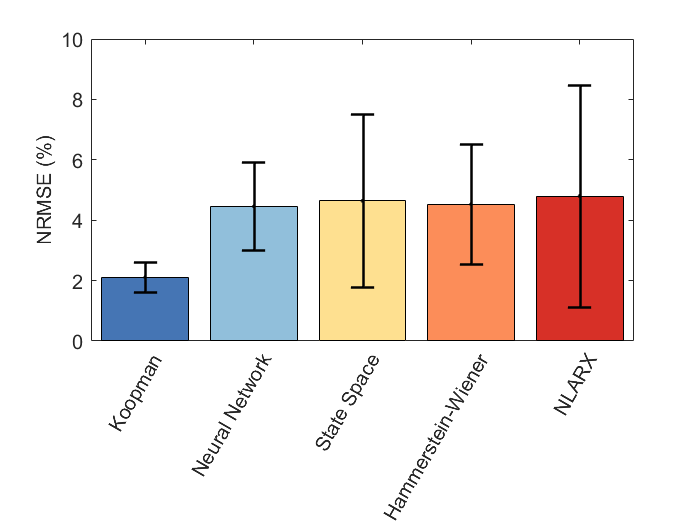
\includegraphics[width=\linewidth]{figures/NRMSE1.png} \\
    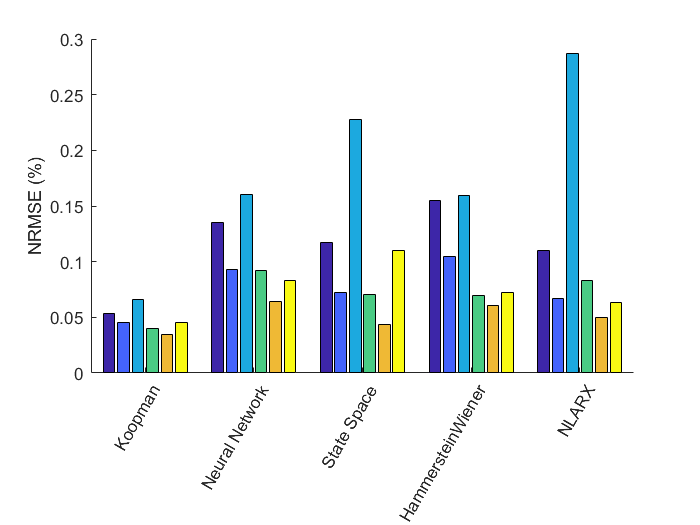
\includegraphics[width=\linewidth]{figures/barStates_ph1.png}
    \caption{PLACEHOLDER: The average NRMSE across all states and all trials for each model (top). The average NRMSE across all trials for each state within each model (bottom).}
    \label{fig:comparison}
\end{figure}

%% TABLE: RMSE results table
\begin{table}[]
    \rowcolors{2}{white}{gray!25}
    \setlength\tabcolsep{5pt} % default value: 6pt
    \centering
    \caption{NRMSE (\%) over all validation trials}
    \begin{tabular}{|c|c|c|c|c|c|c|c|c|c|}
        \hline
        \rowcolor{white} 
        & & \multicolumn{6}{c |}{\textbf{States}} & & \textbf{Std.} \\
        \cline{3-8} \rowcolor{white}
        & \multirow{-2}{*}{\textbf{Model}} & $x_1$ & $x_2$ & $x_3$ & $x_4$ & $x_5$ & $x_6$ & \multirow{-2}{*}{\textbf{Avg.}} & \textbf{Dev.} \\
        \hline
        % RESULTS FOR ROBOT A
        \cellcolor{white} & Koopman & & & & & & & & \\
        \cellcolor{white} & Neural Net & & & & & & & & \\
        \cellcolor{white} & State Space & & & & & & & & \\
        \cellcolor{white} & Ham.-Weiner & & & & & & & & \\
        \multirow{-5}{*}{\cellcolor{white} \rotatebox[origin=c]{90}{\textbf{Robot A}}}
        & NLARX & & & & & & & & \\
        \hline
        % RESULTS FOR ROBOT B
        \cellcolor{white} & Koopman & & & & & & & & \\
        \cellcolor{white} & Neural Net & & & & & & & & \\
        \cellcolor{white} & State Space & & & & & & & & \\
        \cellcolor{white} & Ham.-Weiner & & & & & & & & \\
        \multirow{-5}{*}{\cellcolor{white} \rotatebox[origin=c]{90}{\textbf{Robot B}}}
        & NLARX & & & & & & & & \\
        \hline
    \end{tabular}
    \label{tab:RMSE}
\end{table}